\begin{figure}[htbp]
\centering
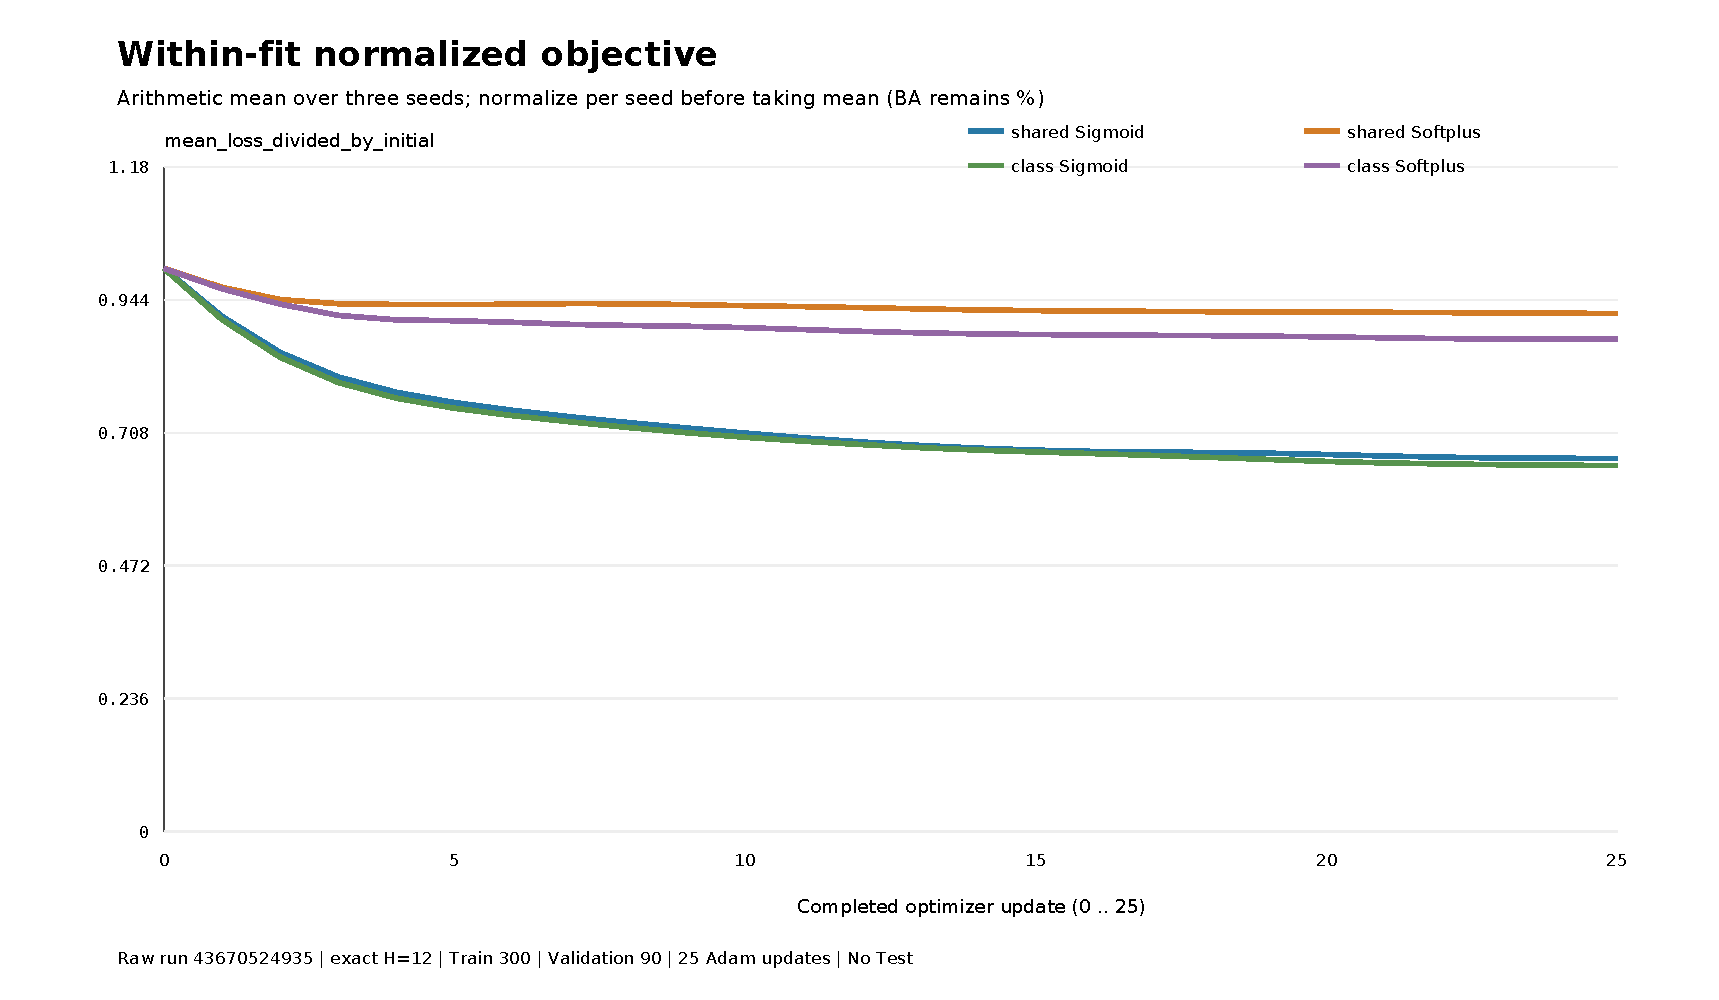
\includegraphics[width=0.98\linewidth]{code/experiments/ch4_loss_controlled_comparison/figures/phase2_tex/phase2_train_loss_relative_dynamics.pdf}
\caption{سیر نسبت تابع زیان به مقدار آغازین هر اجرا، سپس میانگین بر سه بذر. مقیاس نسبی دو تابع زیان قابل تبدیل به مقیاس مطلق مشترک نیست.}
\label{fig:ch4-e13-loss-dynamics}
\end{figure}

\begin{figure}[htbp]
\centering
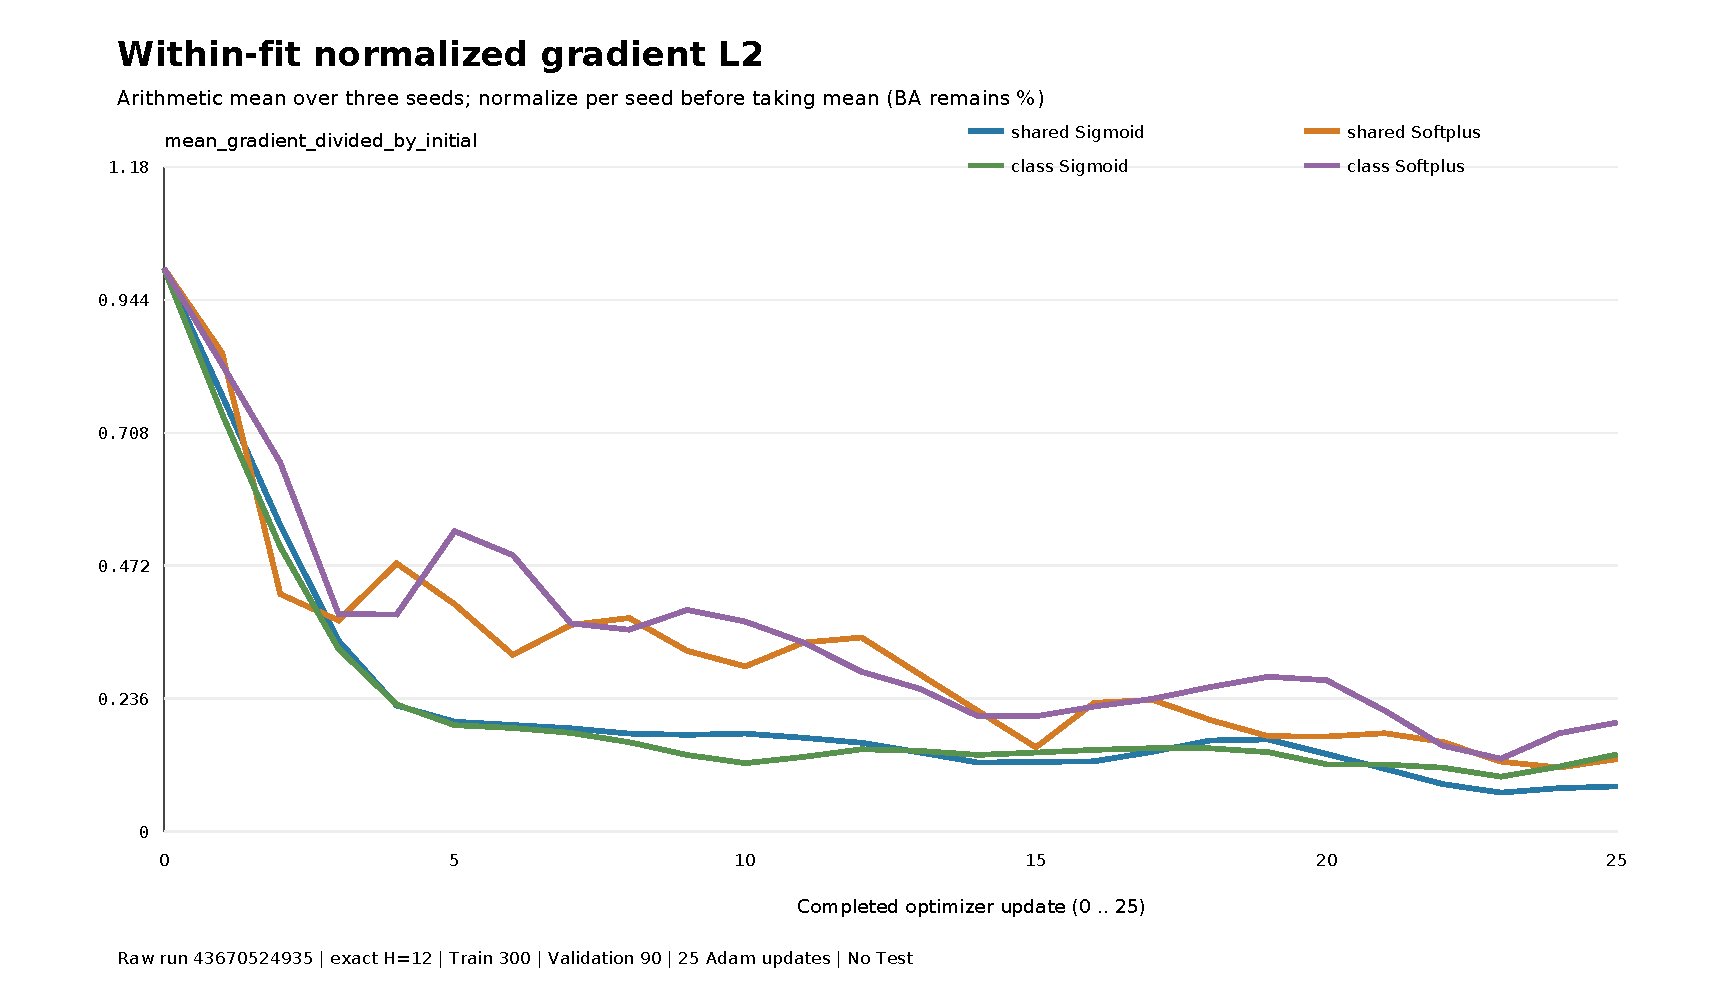
\includegraphics[width=0.98\linewidth]{code/experiments/ch4_loss_controlled_comparison/figures/phase2_tex/phase2_gradient_norm_relative_dynamics.pdf}
\caption{سیر نسبت هنجار گرادیان به مقدار آغازین هر اجرا، سپس میانگین بر سه بذر. نزدیکی نسبی هنجارها اثبات همگرایی به یک بهینه یکسان نیست.}
\label{fig:ch4-e13-gradient-dynamics}
\end{figure}

\begin{figure}[htbp]
\centering
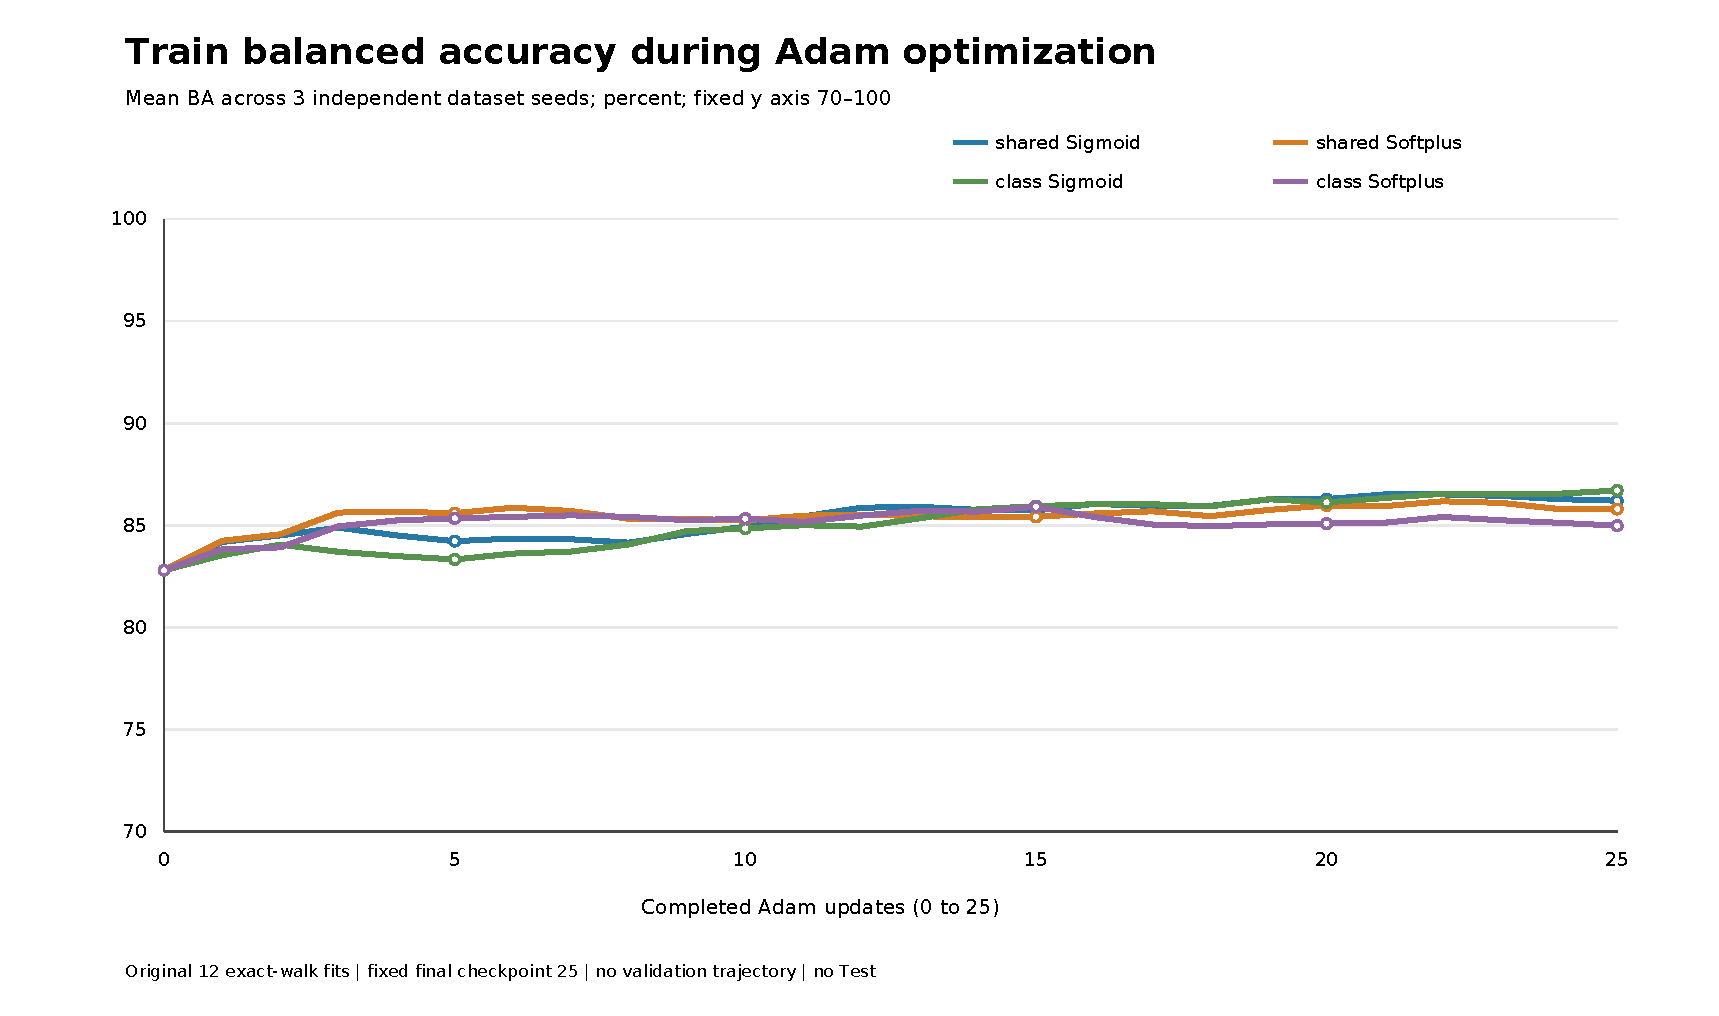
\includegraphics[width=0.98\linewidth]{code/experiments/ch4_loss_controlled_comparison/figures/phase2_tex/figure11_train_BA_y70_100.pdf}
\caption{سیر دقت متوازن آموزش طی ۲۵ به‌روزرسانی آدام؛ محور عمودی عمداً در بازه ۷۰ تا ۱۰۰ درصد ثابت شده تا نزدیکی و تقاطع منحنی‌ها خوانا شود. مقدارها میانگین سه بذرند.}
\label{fig:ch4-e13-train-ba-dynamics}
\end{figure}
